\section{3D nyomtatásról TODO!}

    A 3D nyomtatás maga egy olyan addítív gyártási folyamat mely CAD vagy digitális 3D modellt épít fel
    különböző nyersagokat felhasználva, 3D nyomtatók segítségével. Ma a két legelterjetteb 3D nyomtató
    típus az SLA, mely különleges erre a célra alkalmas gyanta és UV sugarak segítségével építi fel a darabot,
    és az FDM nyomtatók melyek különböző műanyagból készült filamentet használnak nyersanyag gyanánt.
    Mindkét típus bár teljesen más elven működik rétegenként építi fel a darabot egy előre szeletelt
    G-kód-ot követve. A dolgozat általi megvalósítás FDM tipűsú nyomtatókkal foglalkozik.\\ 

    \begin{figure}[H]
        \centering
        \begin{minipage}[t]{0.48\textwidth}
            \centering
            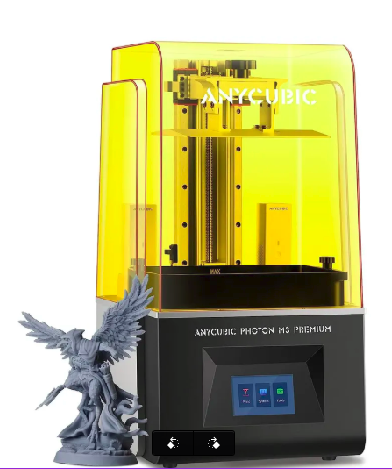
\includegraphics[width=\linewidth,height=6cm,keepaspectratio]{figures/images/literature/SLA.png}
            \caption{SLA nyomtató}
        \end{minipage}\hfill
        \begin{minipage}[t]{0.48\textwidth}
            \centering
            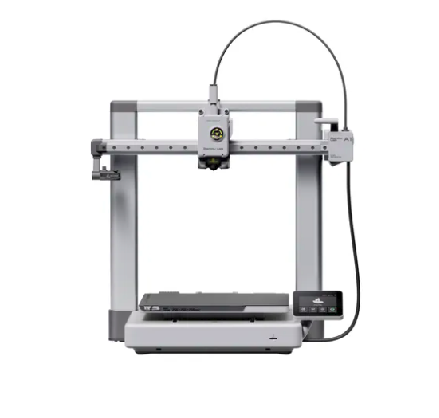
\includegraphics[width=\linewidth,height=6cm,keepaspectratio]{figures/images/literature/FDM.png}
            \caption{FDM nyomtató}
        \end{minipage}
    \end{figure}

    Mint már említettem az FDM 3D nyomtatók különböző filamenteket használnak nyersanyagként, 
    ezekből is több fajta létezik. A legismertebb ezek közül a PLA, mellyel könnyű jól dolgozni,
    főként prototípusok és dísztárgyak nyomtatására alkalmazzuk, mivel az anyag fő gyengesége
    az alacsony olvadáspont (körülbelül 70 celzius fok), és az UV sugarak és a nedvesség és hamar
    kikezdik. Ismertebb filament típusok még a PETG mely jobb mechanikai tulajdonságokkal és ellenálló
    képességgel rendelkezik de még mindig nem az igazi, ha teljes mértékben szükség van mindennemű mechanikai
    ellenállásra, terhelhetőségre akkor ABS-t kell nyomtatnunk, ennek nyomtatása viszont igen igényes, mivel zárt
    teret és állandó hőmérsékletet igényel.Amennyiben pedig flexibilis tárgyakat nyomtatnánk a TPU a mi megoldásunk.


    \begin{figure}[H]
        \centering
        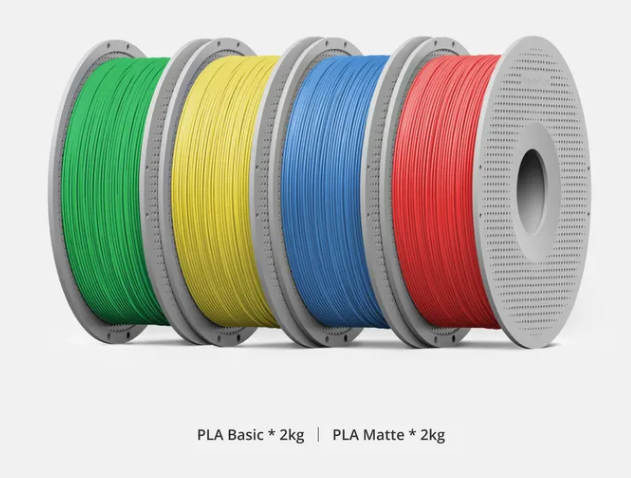
\includegraphics[width=0.6\textwidth]{figures/images/literature/filament.png}
        \caption{Filament tekercsek}
    \end{figure}

        \subsection{Felmerülő hibák és limitációk}
        A 3D nyomtatási folyamat során rengeteg hiba felmerülhet. mely több okból is keletkezhet,
        a nedves anyagtól, a rossz kallibrációig, vagy akár komoly hardver hibáig is. Beszéljünk
        egy kicsit ezen hibákról.

            \subsubsection{Stringing- Avagy szálazás}
                
                \begin{figure}[H]
                    \centering
                    \rotatebox{270}{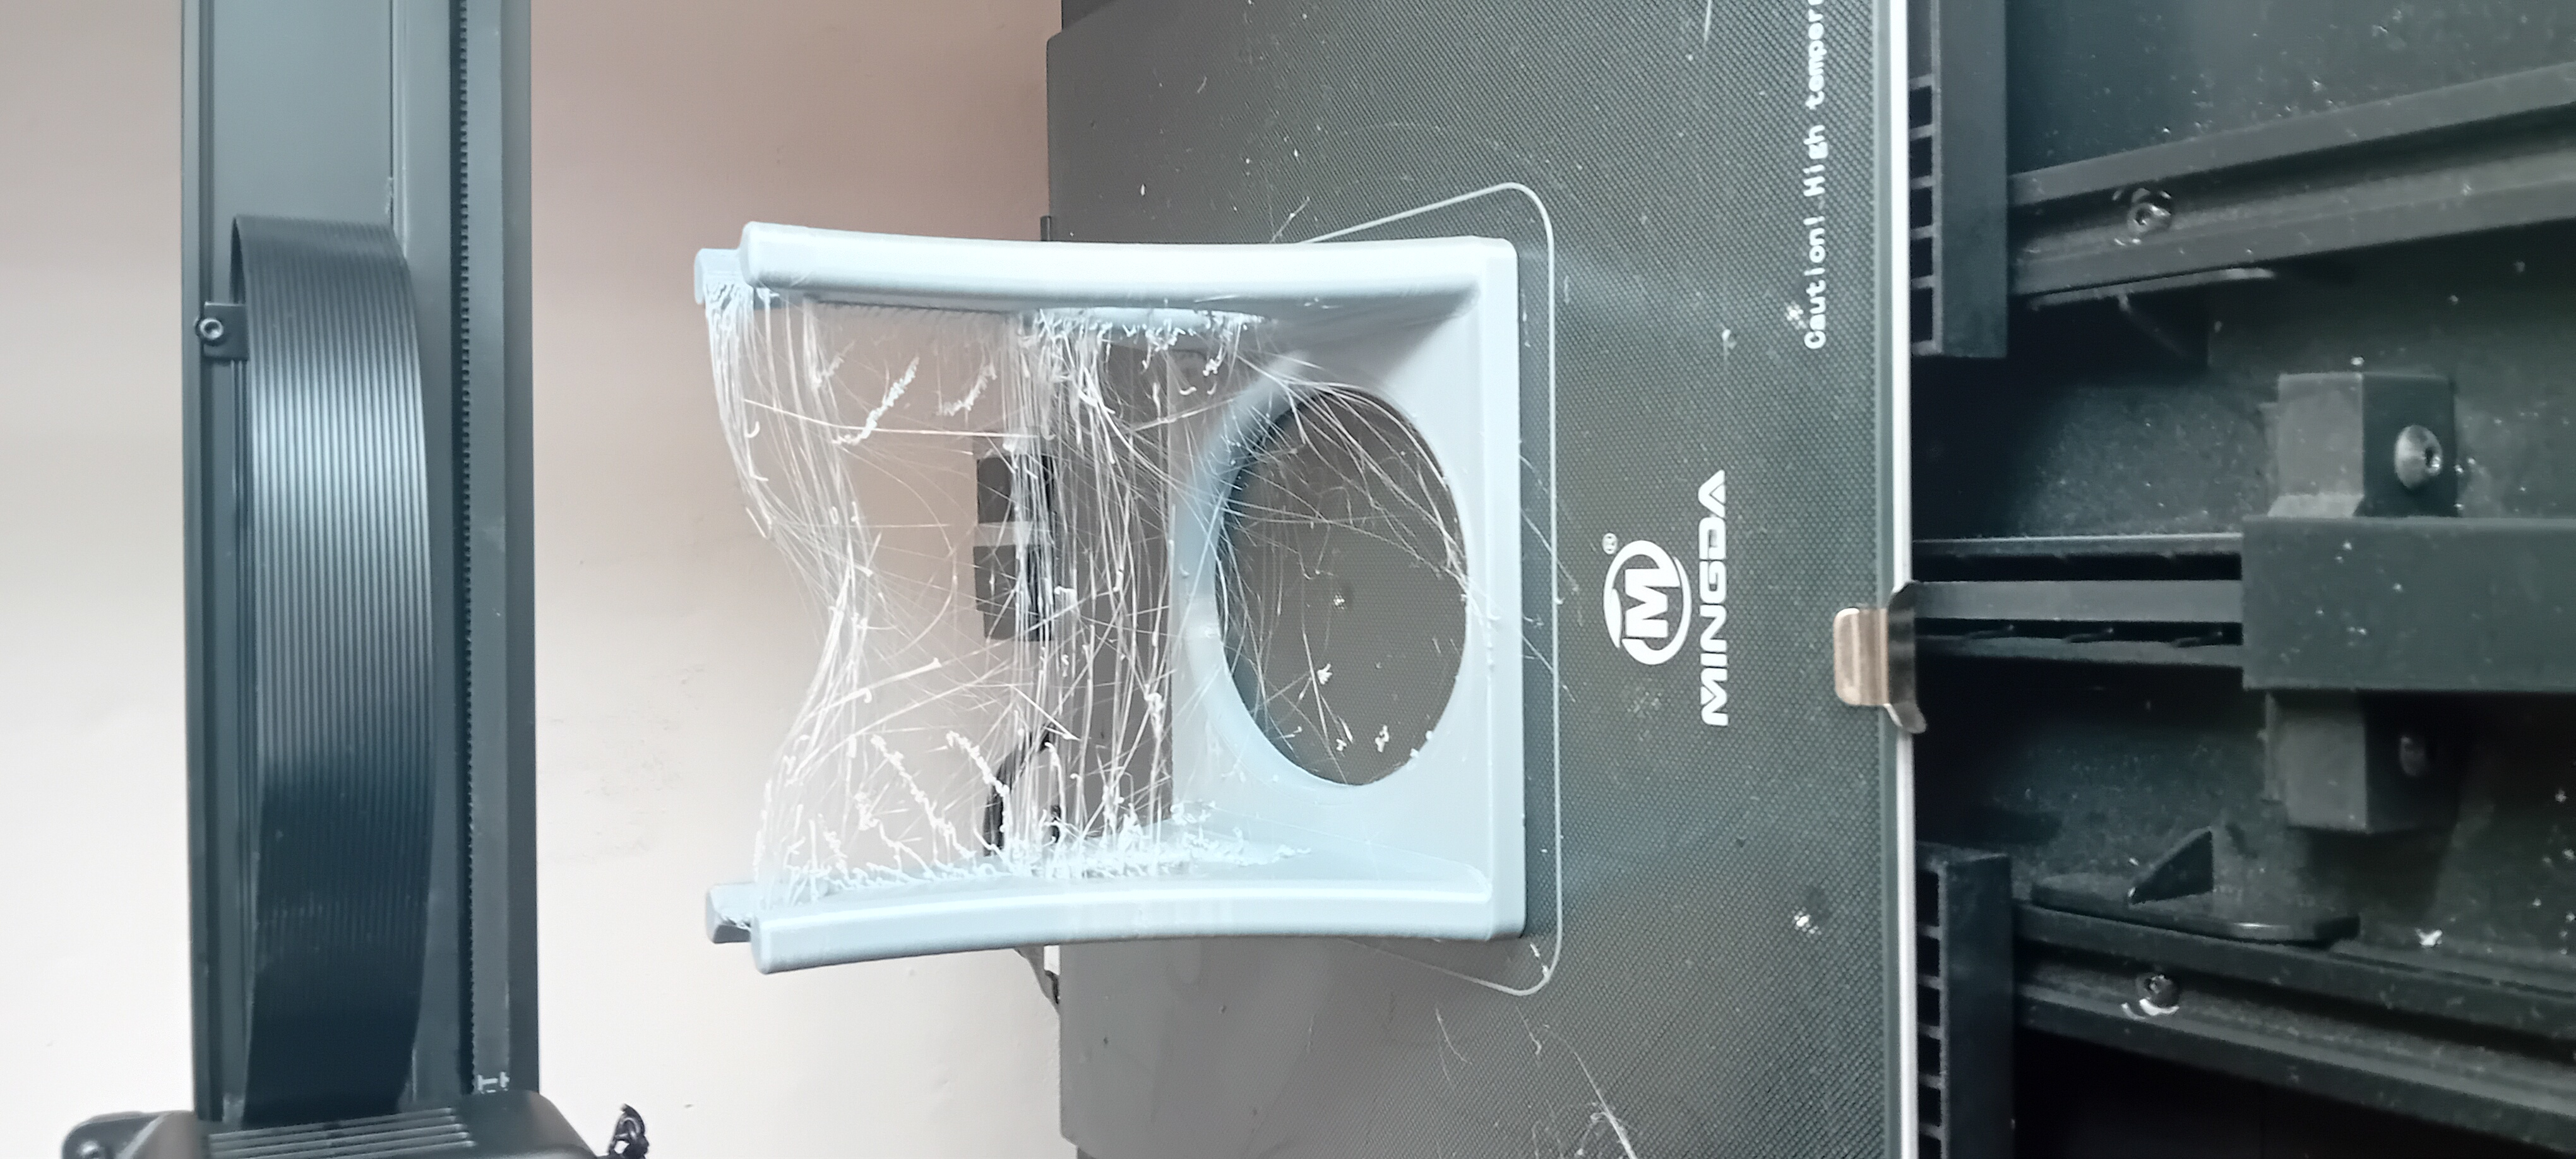
\includegraphics[width=0.6\textwidth]{figures/images/literature/string.jpg}}
                    \caption{Szálazás a nyomtatás végén}
                \end{figure}

            Ez a hiba igen idegesítő tud lenni, mivel rengeteg utómunkát igényel a vékony szálacskák
            eltávolítása, és még úgyis megmarad a nyoma. Több előokozó tényező is lehet. Szeletelés
            során nem megfelelő visszahúzás beállítási érték, nedves filament, túl nagy fúvóka hőmérséklet 
            vagy mocskos fúvóka.


            \subsubsection{Warping- Avagy eltorzulás}

                \begin{figure}[H]
                    \centering
                    {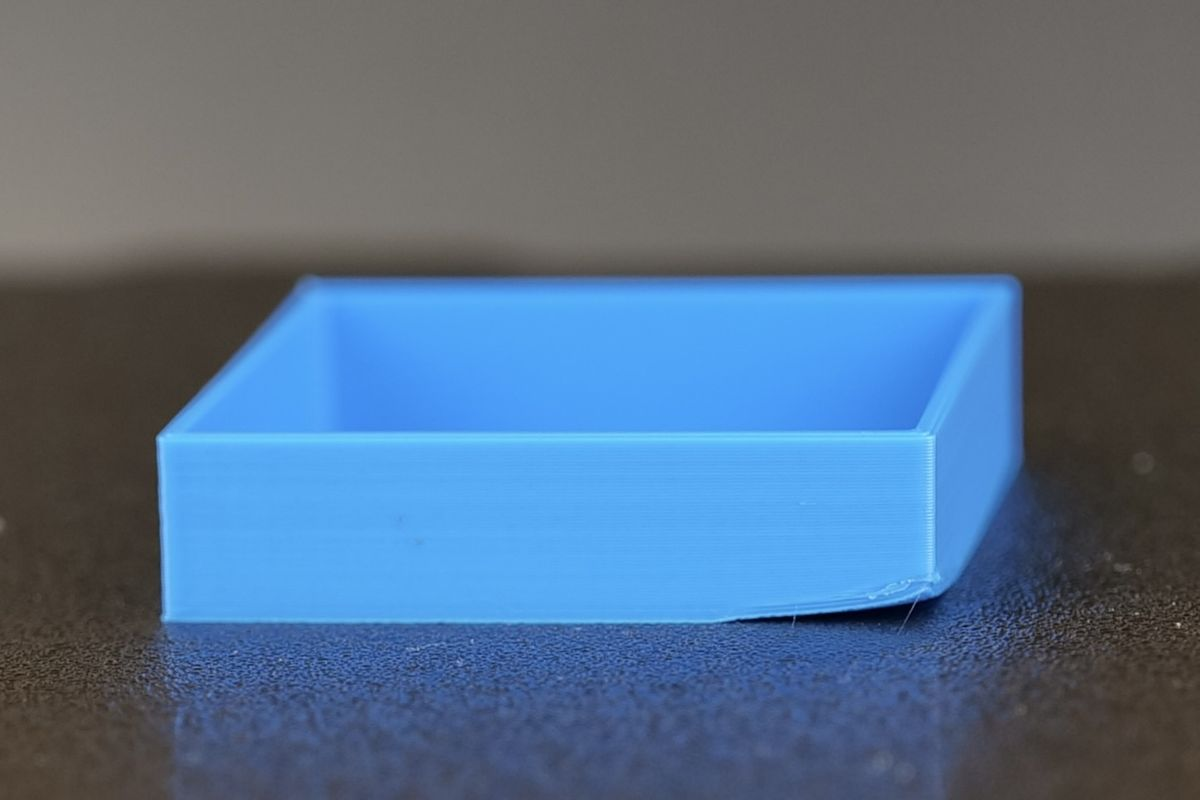
\includegraphics[width=0.6\textwidth]{figures/images/literature/curling_corner.jpg}}
                    \caption{Eltorzult darab}
                \end{figure}

            Eltorzulás legtöbbször akkor jelentkezik, amikor egy darab alján éles szögek találhatóak, 
            például négyzet, vagy egyébb sokszög. Fontos beavatkozó viszont a tárgyasztal hője, tisztasága
            is a megfelelő tapadás fenttartásához. A hiba maga kiküszöbőlhető egy úgynevezett skirt, 
            avagy szoknya alkalmazásával a szeletelőben, mely búnusz tapadást biztosít a sarkakon.

            \subsubsection{Layer shift-Avagy réteg eltolódás}

                \begin{figure}[H]
                    \centering
                    {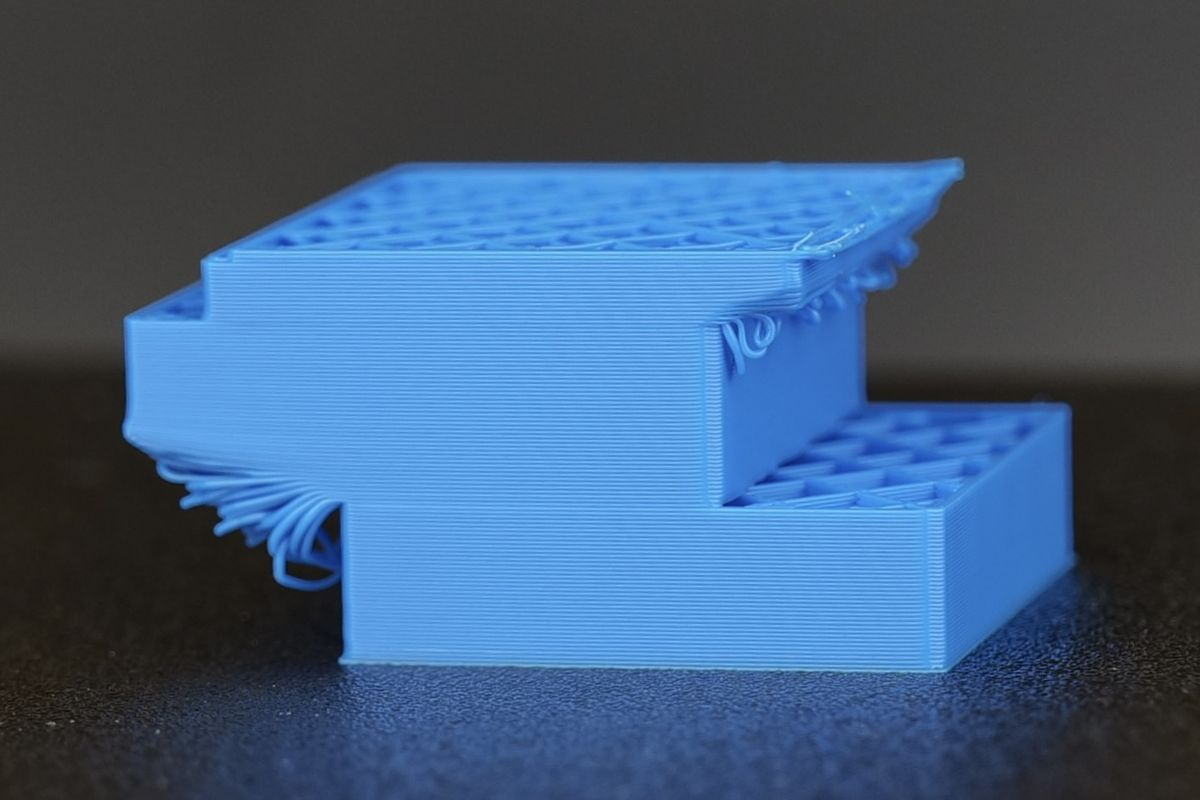
\includegraphics[width=0.6\textwidth]{figures/images/literature/layer_shifts.jpg}}
                    \caption{Elcsúszott rétegek}
                \end{figure}

            A nyomtatott rétegek eltolódása végzetes hiba a darab számára. Főként akkor jelenik meg amikor 
            eltérés van a G-kódban található koordítnáta és a fúvóka világi koordínátái között. Három fő oka
            van, túl nagy nyomtatási sebesség, nem megfelelő Z-offset mely miatt a fúvóka beleakadhat a darabba
            ezzel koordínáta különbséget előídézve, vagy a nyomtatót ért fizikai trauma, esetleg laza sínek 
            vagy merevítők.

            \subsubsection{Under extrusion- Avagy alul extrúdálás}

                \begin{figure}[H]
                    \centering
                    \begin{minipage}[t]{0.48\textwidth}
                        \centering
                        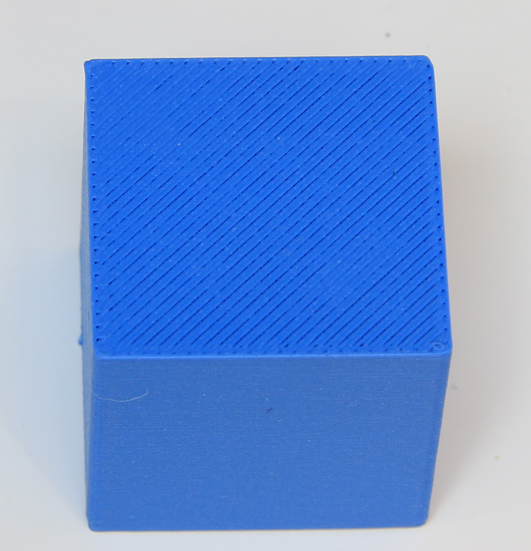
\includegraphics[width=\linewidth,height=6cm,keepaspectratio]{figures/images/literature/underex.png}
                        \caption{Teljes alul extrúdálás}
                    \end{minipage}\hfill
                    \begin{minipage}[t]{0.48\textwidth}
                        \centering
                        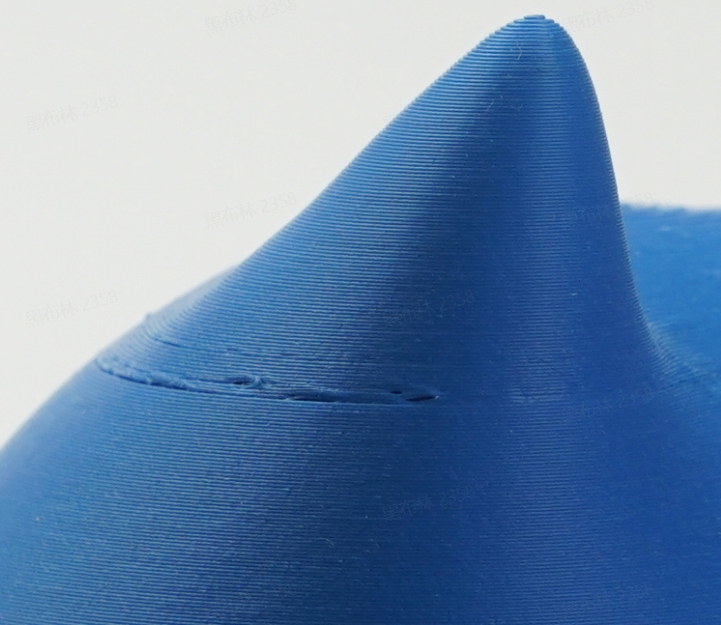
\includegraphics[width=\linewidth,height=6cm,keepaspectratio]{figures/images/literature/lokunderex.jpg}
                        \caption{Lokális alul extrúdálás}
                    \end{minipage}
                \end{figure}
    
            Ezen hibának két külön fajtáját különböztetjük meg, a teljes illetve a lokális alul extrúdálást.
            Ezen hiba okai lehetnek mind hardveres, de előokozhatja nem megfelelő szeletelés is. 
            Főbb előidéző okok közé tartozik, hogyha, eldugul a ptfe cső, vagy idegen test kerül bele, beakadt
            a filament tekercs és nem jút elég a fúvókához, fogaskerék probléma, vagy részleges dugúlás a fúvókában 
            vagy a hotendben. Amennyiben a problémát szoftveres ok váltja ki a Maximum Volumetric speed illetve Flow
            ratio nevű beállításokkal van a probléma. A mai modern nyomtatók már fel vannak szerelve autómatikus adagolás
            kallibrációval, ezzel segítve a felhasználót.

            \subsubsection{Over extrusion- Avagy felül extrúdálás}

                \begin{figure}[H]
                    \centering
                    {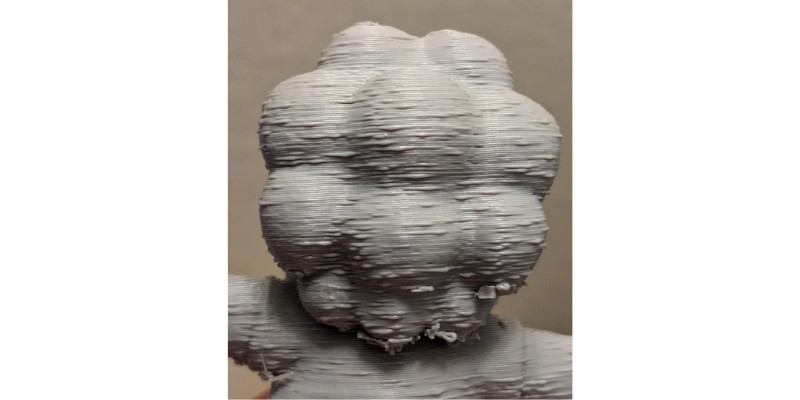
\includegraphics[width=0.6\textwidth]{figures/images/literature/overex.jpg}}
                    \caption{Felül extrúdált darab}
                \end{figure}

            Ugyanazon probléma mint az alul extrúdálás, egy annyi csavarral, hogy itt nem túl kevés anyag jut a 
            fúvókához hanem pont, hogy túl sok.

            \subsubsection{Nozzle Clog- Avagy fúvóka dugulás}

                \begin{figure}[H]
                    \centering
                    {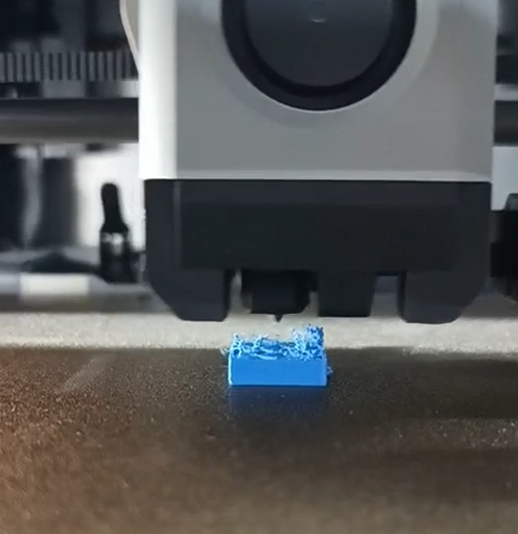
\includegraphics[width=0.6\textwidth]{figures/images/literature/clog.png}}
                    \caption{Nyomtatás közben eldugult fúvóka és darab}
                \end{figure}

            Egy sajnos igen gyakori probléma mely akár a nyomtatónk "életébe" is kerülhet. Legfőbb oka, hogy 
            a filament amikor a ptfe csövön keresztül a forró kamrába, majd pedig a fúvókába jut nem teljesen 
            tiszta, kis por vagy egyébb szennyező anyagok is bekerülnek, melyek a fúvóka dugulását okozhatják. 
            Amennyiben nem vesszük észre hamar az olvadt műanyag felgyülhet a fúvókában és belülről szétfeszíti azt, 
            ezzel jelentős anyagi kárt okozva.

            \subsubsection{Foreign object on the printbed- Avagy idegen tárgy a tárgyasztaklon}

            Ezen hiba se nem hardveres se nem szoftveres hanem szimplán a kezelő figyelmetlensége miatt 
            következik be, akik a tapasztalatomból legtöbbször olyan izgatott a szeletelést követően, 
            hogy elfelejti ellenőrizni, hogy leürítette-e a tárgyasztalt, vagy csak karbantartás után 
            nem pakolt el maga után. Az idegen tárgyak a fúvókában és a fejben súlyos anyagi kárt okozhatnak 
            viszont, hiszen a legtöbb nyomtató nem képes detektálni, ha a tárgyasztal üres vagy sem.
                
                \begin{figure}[H]
                    \centering
                    {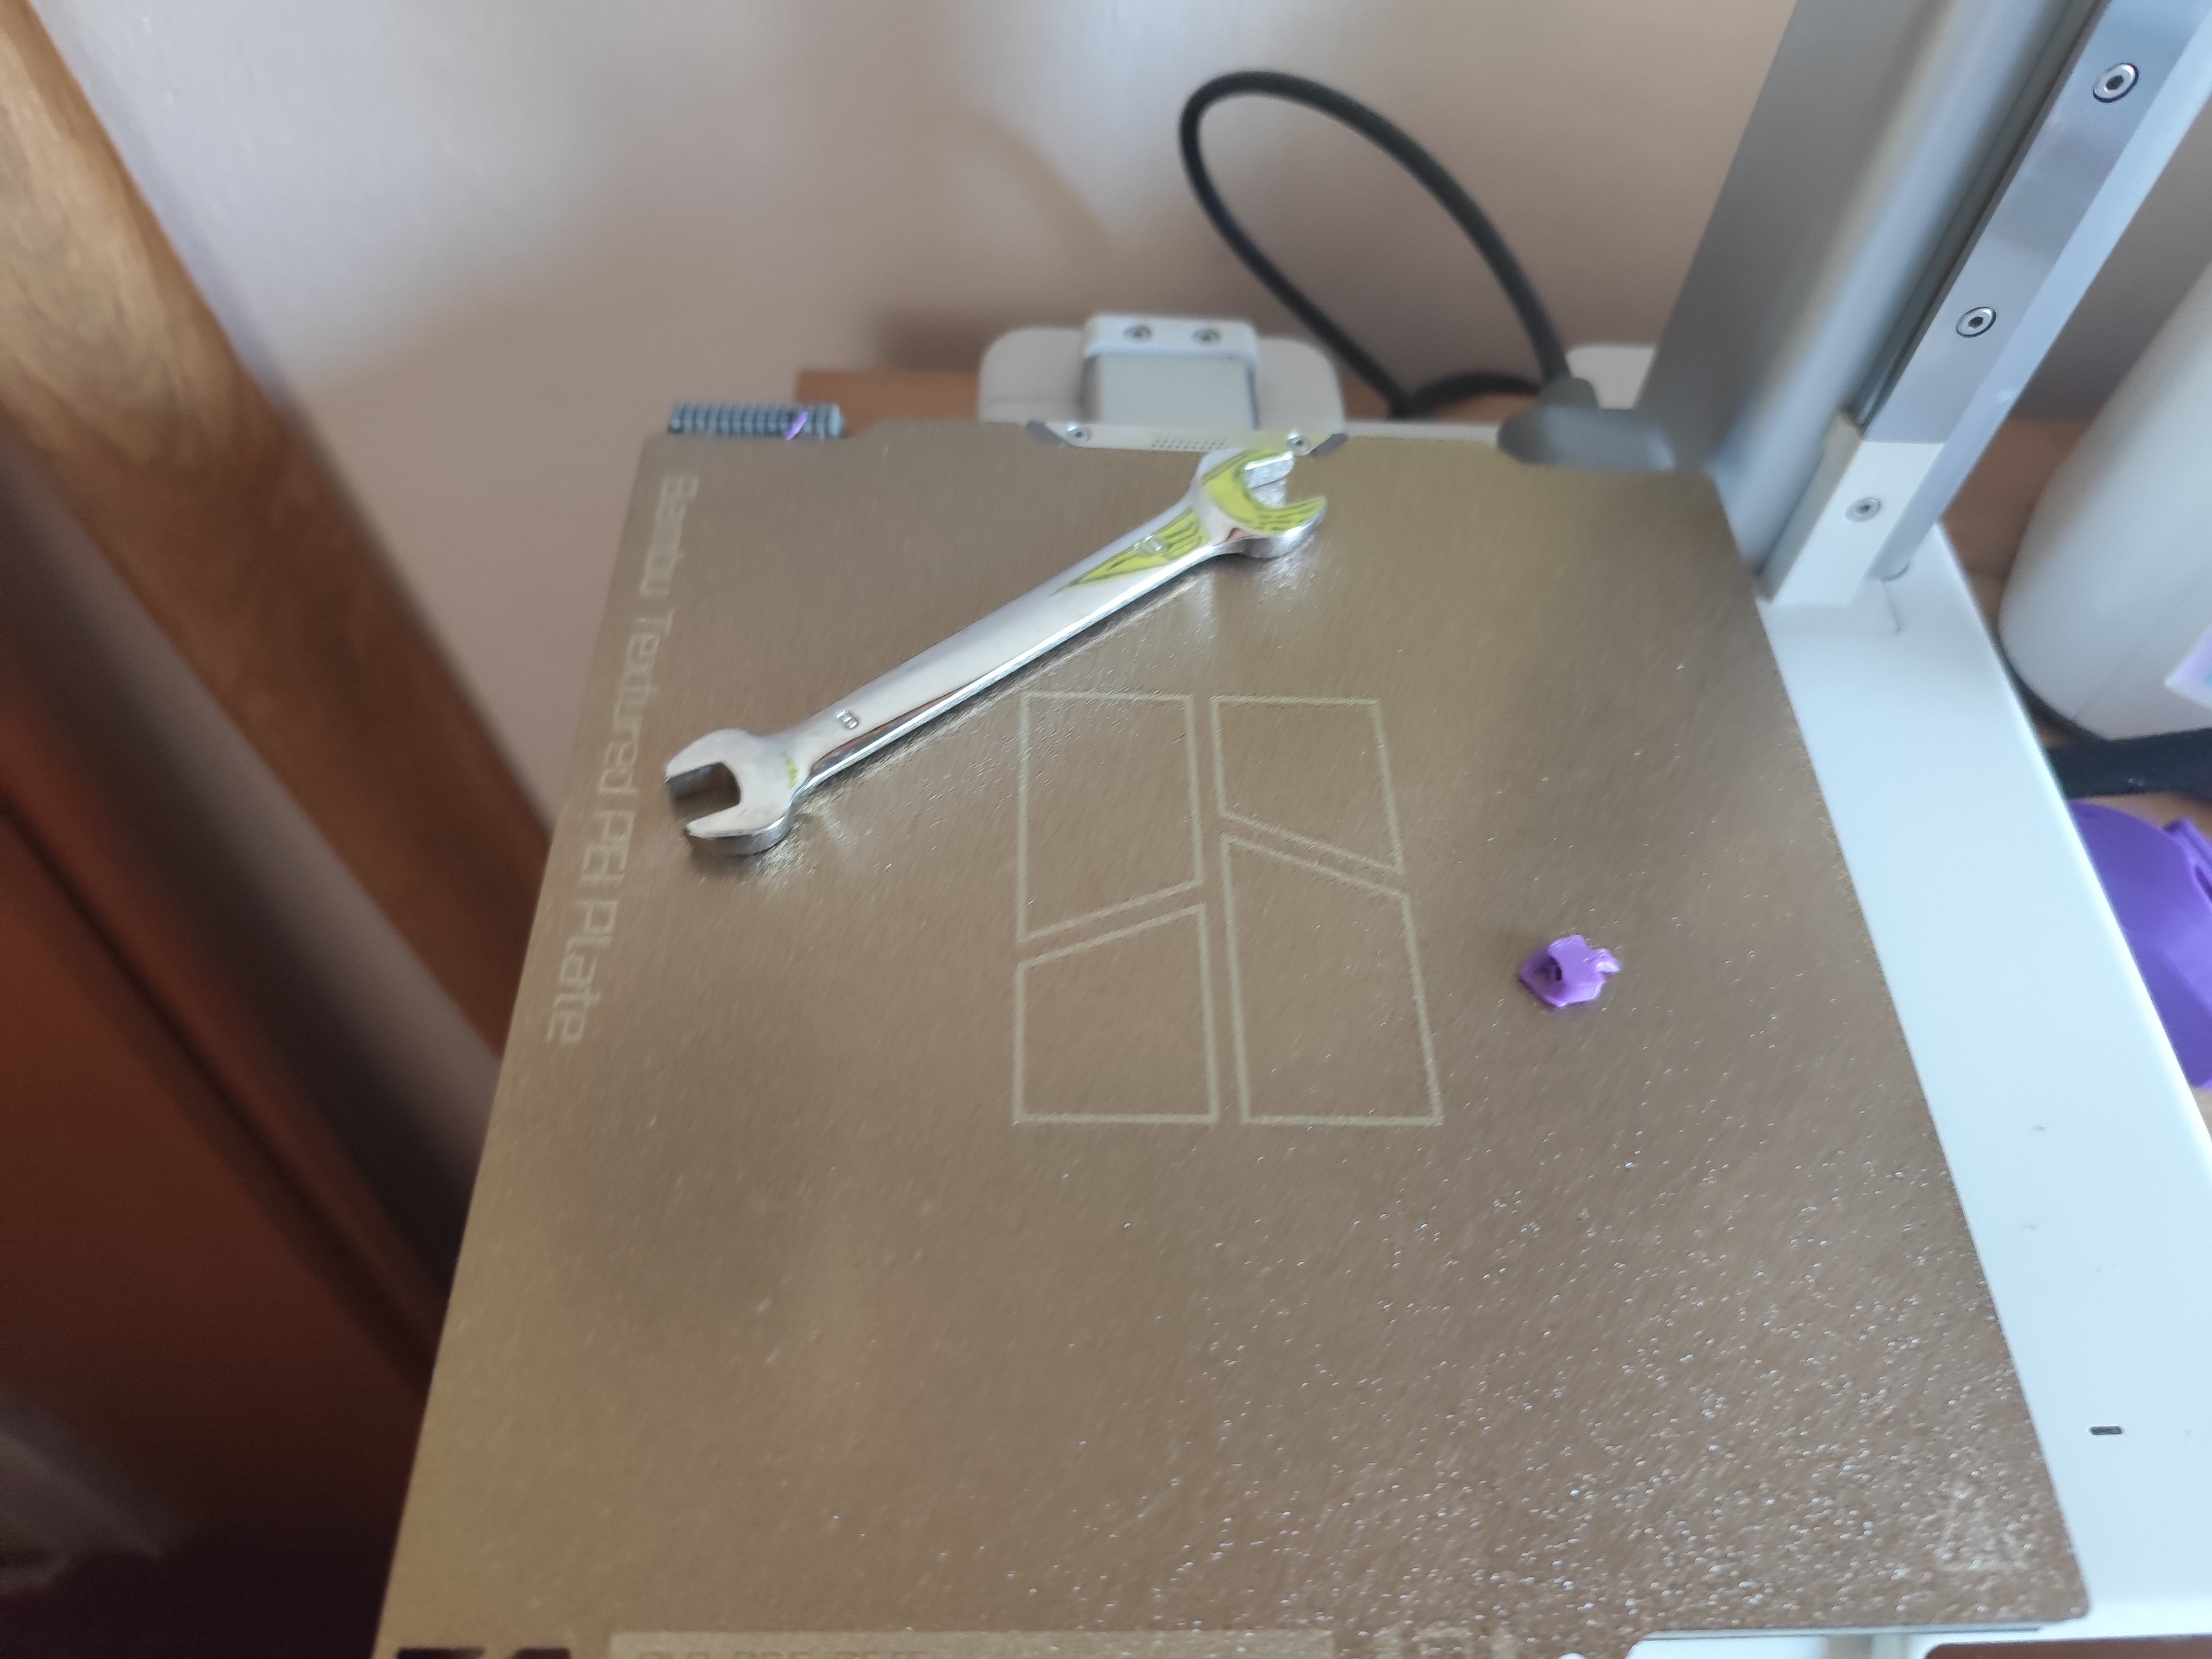
\includegraphics[width=0.6\textwidth]{figures/images/literature/foreign.jpg}}
                    \caption{Figyelmetlenségből a tárgyasztalon hagyott szerszám}
                \end{figure}

            \subsubsection{First layer not sticking- Avagy az első réteg nem tapad}

                \begin{figure}[H]
                    \centering
                    {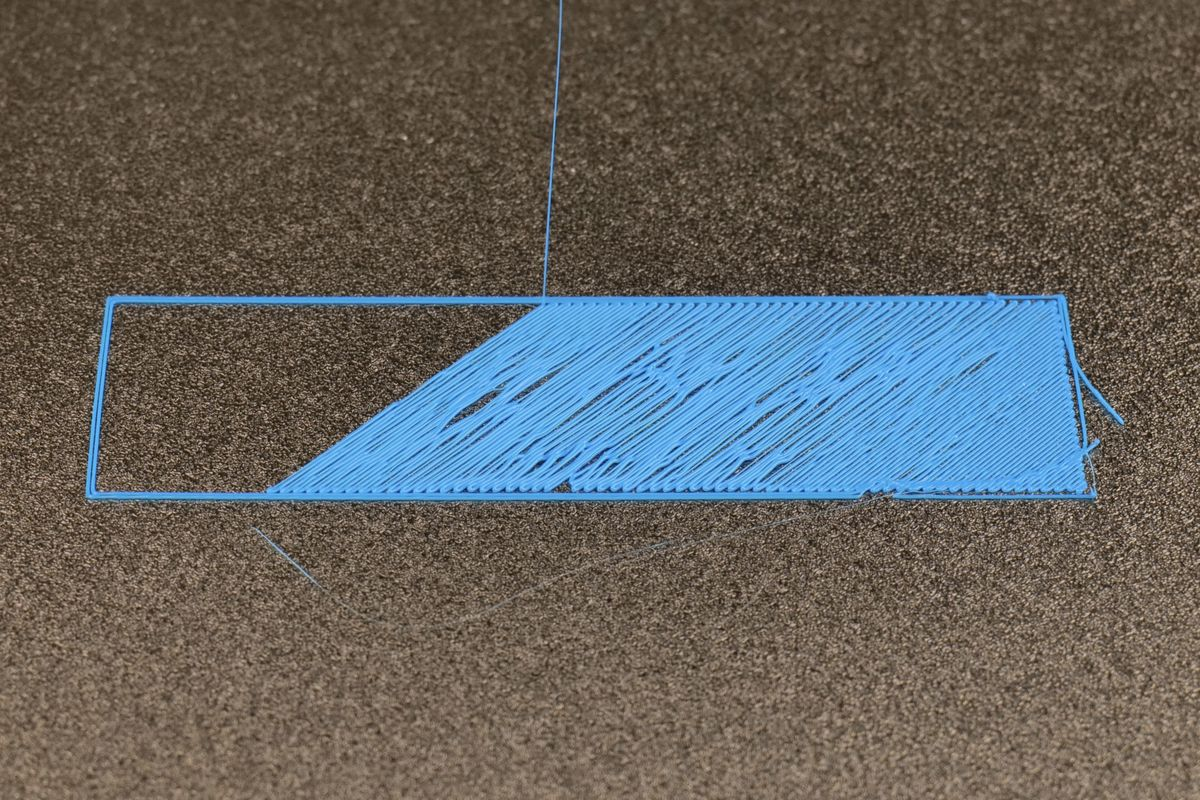
\includegraphics[width=0.6\textwidth]{figures/images/literature/first_layer_not_sticking_to_the_plate.jpg}}
                    \caption{Nem tapadó első réteg}
                \end{figure}

            A 3D nyomtatási folyamat során a legfontosabb mozzanat az első réteg, ha ez nem tapad 
            oda akkor az egész darab kuka, fontos figyelemmel kísérni, amennyiben észrevétlen marad, 
            az Spagettihez, és rengeteg anyag veszteséggel jár. Főbb okai, ha a tárgyasztal nem megfelelő 
            tisztaságú, rossz fúvóka tárgyasztal távolság (Z-offset), vagy rossz asztal szintezés. Könnnyen 
            elkerülhető a megfelelő beállításokkal és a tárgyasztal karban-és tisztán tartásával.

            \subsubsection{Spagetti- Avagy az anyag a levegőbe adagolódik}

            Rengeteg oka lehet, de a legfőbb előokozója, ha az első réteg nyomtatási folyamata sikertelennek 
            bizonyult, a fúvókát ez nem érdekli, ő követi a G-kód által megadott utasításokat és addig nyomja a 
            levegőbe az anyagot, ameddig a végére nem ér, vagy a kezelő azt meg nem állítja. 
            Fontos kiemelni, hogy a tapadás elvesztése a nyomtatási folyamat bármely pillanatában bekövetkezhet, 
            amennyiben nem megfelelő support beállításokat alkamaztunk a szeletelőben, vagy éppen a supportok 
            engedik el a tárgyasztalt, ezzel védtelenül hagyva a darabot.

                \begin{figure}[H]
                    \centering
                    \rotatebox{270}{
\includegraphics[width=0.6\textwidth]{figures/images/literature/spagetti.jpg}}
                    \caption{Hibás nyomtatást követő spagetti halmaz}
                \end{figure}

